\chapter{Analysis of Effective Field Theory Interactions in LZ}



\begin{figure}[!htbp]%
\centering
\begin{tikzpicture}
\centering
  \begin{groupplot}[view={0}{90},
    group style = {group size = 2 by 4,
                   vertical sep=1.5cm,
                   horizontal sep=2.0cm}]
    
    \pgfplotsforeachungrouped \x in {1,3,4,5,6,7,8,9}{
     \edef\tmp{
        \noexpand \nextgroupplot[
                                xlabel=Mass (MeV),
                                ylabel=$({c}^{s}_{\x}\times{m}^{2}_{w})^{2}$,
                                mark size=0pt,
                                width=0.45\textwidth,
                                height=5.5cm,
                                xmode=log,
                                ymode=log,
                                x label style={at={(axis description cs:0.75,-0.1)},anchor=near ticklabel},
                                y label style={at={(axis description cs:-0.13,.75)},anchor=near ticklabel},
                                ]
            
            \noexpand \addplot[blue, name path = xenon100] table[]
                      {Data/HENR/Xenon100/O\x.dat};
                        
            
            \noexpand \addplot[green, opacity = 0.4, name path = ns1] table[x=mass, y=ns1]
                      {Data/HENR/Projected_Sensitivity/Results/O0\x.dat};
                      
            \noexpand \addplot[green, opacity = 0.4, name path = ps1] table[x=mass, y=ps1]
                      {Data/HENR/Projected_Sensitivity/Results/O0\x.dat};
                      
            \noexpand \addplot[yellow, opacity = 0.4, name path = ps2] table[x=mass, y=ps2]
                      {Data/HENR/Projected_Sensitivity/Results/O0\x.dat};
                      
            \noexpand \addplot[green, opacity = 0.4, forget plot] fill between[of=ns1 and ps1];
            \noexpand \addplot[yellow, opacity = 0.4, forget plot] fill between[of=ps1 and ps2];
            
            \noexpand \addplot[black, name path = exp] table[x=mass, y=exp]
                      {Data/HENR/Projected_Sensitivity/Results/O0\x.dat};
            
            %\noexpand \addplot[black, dashed, name path = exp] table[x=mass, y=cl]
            %          {Data/HENR/Projected_Sensitivity/Results/O0\x.dat};
                     
        }
        \tmp 
        }
  \end{groupplot}
\end{tikzpicture}
\caption{}
\label{fig:EFT_Result_Projected_Sensitivity_1}
\end{figure}



\begin{figure}[!htbp]%
\centering
\begin{tikzpicture}
\centering
  \begin{groupplot}[view={0}{90},
    group style = {group size = 2 by 3,
                   vertical sep=1.5cm,
                   horizontal sep=2.0cm}]
    
    \pgfplotsforeachungrouped \x in {10,11,12,13,14,15}{
     \edef\tmp{
        \noexpand \nextgroupplot[
                                xlabel=Mass (MeV),
                                ylabel=$({c}^{s}_{\x}\times{m}^{2}_{w})^{2}$,
                                mark size=0pt,
                                width=0.45\textwidth,
                                height=5.5cm,
                                xmode=log,
                                ymode=log,
                                x label style={at={(axis description cs:0.75,-0.1)},anchor=near ticklabel},
                                y label style={at={(axis description cs:-0.13,.75)},anchor=near ticklabel},
                                ]
            
            \noexpand \addplot[blue, name path = xenon100] table[]
                      {Data/HENR/Xenon100/O\x.dat};
                        
            \noexpand \addplot[green, opacity = 0.4, name path = ns1] table[x=mass, y=ns1]
                      {Data/HENR/Projected_Sensitivity/Results/O\x.dat};
                      
            \noexpand \addplot[green, opacity = 0.4, name path = ps1] table[x=mass, y=ps1]
                      {Data/HENR/Projected_Sensitivity/Results/O\x.dat};
                      
            \noexpand \addplot[yellow, opacity = 0.4, name path = ps2] table[x=mass, y=ps2]
                      {Data/HENR/Projected_Sensitivity/Results/O\x.dat};
                      
            \noexpand \addplot[green, opacity = 0.4, forget plot] fill between[of=ns1 and ps1];
            \noexpand \addplot[yellow, opacity = 0.4, forget plot] fill between[of=ps1 and ps2];
            
            \noexpand \addplot[black, name path = exp] table[x=mass, y=exp]
                      {Data/HENR/Projected_Sensitivity/Results/O\x.dat};
            
            %\noexpand \addplot[black, dashed, name path = exp] table[x=mass, y=cl]
            %          {Data/HENR/Projected_Sensitivity/Results/O\x.dat};
                     
        }
        \tmp 
        }
  \end{groupplot}
\end{tikzpicture}
\caption{}
\label{fig:EFT_Result_Projected_Sensitivity_2}
\end{figure}

\section{Signal Model}
\par
The actual signal model is actually produced by taking a theoretical event rate spectrum (produced by a Mathematica package - DMFormFactor - developed by XXX) and applying the analysis acceptance and detector response.
Passing through LZLama or PdfMaker, this turns the above into event observable - S1 and LogS2).
\par
DMFormFactor takes performs the calculations described previously.
Each Xenon isotope is evaluated separately and is weighted by the Xenon abundance before being added together to produce an energy spectrum.
As mentioned previously, the energy spectrum is dependant upon the choice of coupling and the WIMP mass.
\par
The choice has been made to perform analysis in iso-scalar rather than proton-neutron. 
There is always an argument that one approach is more appropriate than the other
\par
In table \ref{tab:DMFormFactor_parameters} the parameters used for this are shown.
The majority of these values are to match those from previous studies and the Dark Matter community standards.

\begin{table}[]
    \centering
    \begin{tabular}{c|c}
        Parameter   & Value  \\ \hline
        $\nu_0$     & 220$km s^{-1}$ \\
        $\nu_{esc}$ & 544$km s^{-1}$ \\
        $\rho_{0}$     & 0.3 $GeV/cm^{3}$ \\
        $\nu_E$     & 245 $km s^{-1}$ 
    \end{tabular}
    \caption{DMFormFactor parameters used for the standard halo model. CITE XXX}
    \label{tab:DMFormFactor_parameters}
\end{table}


\par
A subset of the recoil spectra calculated are shown in Figures \ref{fig:HENR_Spin_Recoil_Spectrum} and \ref{fig:HENR_NotSpin_Recoil_Spectrum}.
The masses for which the energy spectra were calculated were;
[5, 7, 10, 12, 14, 21, 33, 50, 100, 200, 400, 1000, 4000] GeV all of which can be seen in Annex XXX.
The reason for this is that the shape of the limit produced is fairly well understood, so only a subset of WIMP masses are needed.

\newcommand{\allrecoiloperators}{01s,03s,04s,05s,06s,07s,08s,09s,10s,11s,12s,13s,14s,15s}
\newcommand{\spinrecoiloperators}{01s,04s,06s,07s,09s,10s,11s,14s}
\newcommand{\roguerecoiloperators}{03s,05s,08s,12s,13s,15s}

\begin{figure}[!htbp]%
\centering
\begin{tikzpicture}
\centering
  \begin{groupplot}[view={0}{90},
    group style = {group size = 2 by 1}]
    \nextgroupplot[
    xlabel=Recoil Energy (keV),
    ylabel=Differential Rate (kg/day/keV),
    legend pos=north east,
    mark size=0pt,
    xmin=1, xmax=400, xmode=log,
    ymin=1e-14, ymax=1e3, ymode=log]
    \foreach \henrop in \spinrecoiloperators{
                \addplot 
                    table
                    %{Data/HENR/Signal/Recoils/dRdEr_EFT_O01s_m5GeV_0.txt};
                    {Data/HENR/Signal/Recoils/dRdEr_EFT_O\henrop_m5GeV_0.dat};
            }
    \nextgroupplot[
    xlabel=Recoil Energy (keV),
    legend pos=north east,
    mark size=0pt,
    xmin=1, xmax=400, xmode=log,
    ymin=1e-14, ymax=1e3, ymode=log]
    \foreach \henrop in \spinrecoiloperators{
                \addplot
                    table
                    %{Data/HENR/Signal/Recoils/dRdEr_EFT_O01s_m5GeV_0.txt};
                    {Data/HENR/Signal/Recoils/dRdEr_EFT_O\henrop_m21GeV_0.dat};
            }
  \end{groupplot}
\end{tikzpicture}
\caption{Literal Aids
\textbf{Left:} $Gd^{156}$ de-excitation path.
\textbf{Right:} $Gd^{158}$ de-excitation path.
}
\label{fig:HENR_Spin_Recoil_Spectrum}
\end{figure}

\begin{figure}[!htbp]%
\centering
\begin{tikzpicture}
\centering
  \begin{groupplot}[view={0}{90},
    group style = {group size = 2 by 1}]
    \nextgroupplot[
    xlabel=Recoil Energy (keV),
    ylabel=Differential Rate (kg/day/keV),
    legend pos=north east,
    mark size=0pt,
    xmin=1, xmax=400, xmode=log,
    ymin=1e-14, ymax=1e3, ymode=log]
    \foreach \henrop in \roguerecoiloperators{
                \addplot 
                    table
                    %{Data/HENR/Signal/Recoils/dRdEr_EFT_O01s_m5GeV_0.txt};
                    {Data/HENR/Signal/Recoils/dRdEr_EFT_O\henrop_m5GeV_0.dat};
            }
    \nextgroupplot[
    xlabel=Recoil Energy (keV),
    legend pos=north east,
    mark size=0pt,
    xmin=1, xmax=400, xmode=log,
    ymin=1e-14, ymax=1e3, ymode=log]
    \foreach \henrop in \roguerecoiloperators{
                \addplot
                    table
                    %{Data/HENR/Signal/Recoils/dRdEr_EFT_O01s_m5GeV_0.txt};
                    {Data/HENR/Signal/Recoils/dRdEr_EFT_O\henrop_m5GeV_0.dat};
            }
  \end{groupplot}
\end{tikzpicture}
\caption{Literal Aids
\textbf{Left:} $Gd^{156}$ de-excitation path.
\textbf{Right:} $Gd^{158}$ de-excitation path.
}
\label{fig:HENR_NotSpin_Recoil_Spectrum}
\end{figure}

\par
When performing this analysis, an important choice is the coupling choice.


\paragraph{Copied from Billy}
\par
To allow for ease of comparison to previous limit setting on the inelastic36
WIMP-nucleon EFT operators by the XENON collaboration [? ], this analysis was conducted in the isoscalar basis.37
In the isoscalar basis, the charge densities of the nucleons are effectively averaged such that the interaction becomes38
indiscriminate to the type of nucleon involved, even though both the isoscalar and proton-neutron basis provide insight.39
For this WIMP-nucleon EFT, the UV scale governing the physics is far higher than the energies that are probed in the40
experiment. At these lower energies, the UV interactions have to be reduced to effective ones, which is done at the u,41
d and s quark level. The assumption is made that the couplings to each quark at these scales are roughly equivalent.42
Therefore the mass differences of these quarks are negligible at the high-energy scale of the underlying physics, and the43
interaction would be isoscalar. By performing this analysis in the isoscalar basis, it is possible to test this assumption’s44
validity. Additionally, by using either an isoscalar or isovector basis, the target’s nuclear state can be considered as45
isospin symmetric; a property of the strong force that can aid in simplifying the analysis.

\begin{figure}
    \centering
    
\includegraphics[width=0.5\textwidth]{Figures/Placeholder.png}
    \caption{Integrated rate for each operator for a 1000GeV DM particle}
    \label{fig:operator_integrated_rate}
\end{figure}

\begin{table}[]
    \centering
    \begin{tabular}{c|c}
        Parameter   & Value  \\ \hline
        $g_{1}$     & 0.119 \\
        $g_{2}$     & 79.1  
    \end{tabular}
    \caption{Key detector parameters for the LXe-TPC parameters as used in \cite{LZ_projected_sensitivity_paper_ref}}
    \label{tab:projected_sensitivity_detector_parameters}
\end{table}

\section{Background Model}
\par
The backgrounds were only considered up to 240keV as that is the highest dataset that NEST has been able to calibrate to, and so was limited to this to avoid having to extrapolate.
This higher energy backgrounds are the same as those used for the LZ projected sensitivity paper \cite{LZ_projected_sensitivity_paper_ref} but with the maximum energy probed being increased (from 50 to 240) which increased the S1 phd from 80 to 500.

\par
For this work, only the Detector components were required to be re-analyised as the spectras were not previous probed to the higher energies, however, all of the other sources were.
The processes followed the scheme described in \cite{LZ_projected_sensitivity_paper_ref} but is summarised below;



\par
The resultant normalised-to-rate energy spectra for each background considered are shown in Figure XXX.

\begin{figure}[!htbp]%
\centering
    \begin{tikzpicture}
    \centering
        \begin{groupplot}[view={0}{90},
            group style = {group size = 2 by 1}]
            \nextgroupplot[
            width=0.5\textwidth, height=8cm,
            xlabel=Recoil Energy (keV),
            ylabel=Differential Rate (kg/day/keV),
            legend pos=north east,
            mark size=0pt,
            xmin=0, xmax=2700,
            ymode=log]
                \addplot
                    table[x=Energy,y=Rate]
                    {Data/HENR/Projected_Sensitivity/Background_Rates/detector_er.dat};
      %          \addlegendentry{Det. + Sur. + Env.};
      %         \addplot
      %             table[x=Energy,y=Rate]
      %             {Data/HENR/Projected_Sensitivity/Background_Rates/Xe136.dat};
      %          \addlegendentry{${}^{136}$Xe}
      %         \addplot
      %             table[x=Energy,y=Rate]
      %             {Data/HENR/Projected_Sensitivity/Background_Rates/Rn222.dat};
      %          \addlegendentry{${}^{222}$Rn};
      %         \addplot
      %             table[x=Energy,y=Rate]
      %             {Data/HENR/Projected_Sensitivity/Background_Rates/Rn220.dat};
      %          \addlegendentry{${}^{220}$Rn};
      %         \addplot
      %             table[x=Energy,y=Rate]
      %             {Data/HENR/Projected_Sensitivity/Background_Rates/Solar.dat};
      %          \addlegendentry{Solar $\nu$};
      %         \addplot
      %             table[x=Energy,y=Rate]
      %                {Data/HENR/Projected_Sensitivity/Background_Rates/Kr85.dat};
      %          \addlegendentry{${}^{85}$Kr};
                  
            \nextgroupplot[
            width=0.5\textwidth, height=8cm,
            xlabel=Recoil Energy (keV),
            yticklabel pos=right,
            legend pos=north east,
            mark size=0pt,
            xmin=0, xmax=250,
            ymin=1e-12, ymax=,
            ymode=log]
                \addplot
                    table[x=Energy,y=Rate]
                    {Data/HENR/Projected_Sensitivity/Background_Rates/detector_nr.dat};
                \addlegendentry{Det. + Sur. + Env.};
           %     \addplot
           %         table[x=Energy,y=Rate]
           %         {Data/HENR/Projected_Sensitivity/Background_Rates/atm.dat};
           %     \addlegendentry{Atm};
           %     \addplot
           %         table[x=Energy,y=Rate]
           %         {Data/HENR/Projected_Sensitivity/Background_Rates/DSN_DiffRate.dat};
           %     \addlegendentry{DSN};
           %     \addplot
           %         table[x=Energy,y=Rate]
           %         {Data/HENR/Projected_Sensitivity/Background_Rates/hep.dat};
           %     \addlegendentry{hep};
           %     \addplot
           %         table[x=Energy,y=Rate]
           %         {Data/HENR/Projected_Sensitivity/Background_Rates/B8.dat};
           %     \addlegendentry{${}^{8}$B}
        
        \end{groupplot}
    \end{tikzpicture}
    \caption{Backgrounds considered in the PLR}
    \label{fig:sensitivity_paper_backgrounds}
\end{figure}

\par
Of particular note is the lack of inclusion of $\gamma$-X events.
In order to account for them, a more advanced PLR is required which takes into account interaction position \cite{billyboxer_thesis_ref, LUX_RUN4_EFT_2021}.


\par
Additionally, up to this point it is reasonable to assume that the background is flat as this is below the energy of Xe decays and shells.



\begin{equation}
    \sigma_{SI} = C \times \frac{N_{ob}}{N_{exo}} \times \frac{1}{\frac{1}{\nu_{\chi,N}} \times \pi \times \mu_{Higgs}}
\end{equation}
Here $C$ is the conversion from $cm^{2}$ to $GeV$, $\mu_{Higgs}$ is the vaccumn expectation, $\nu_{\chi,N}$ is the reduced mass.



%\section{LZ MDC3}
\par
Mock-Data Challenge 3 was the third and final simulation campaign prior to the availability of real data.
This campaign was designed to test the entirety of analysis framework to ensure data-readiness.

\par
As this simulation dataset was performed before the availability of real-data naturally some of the detector parameters used in the simulation are wrong.

\par
Something about PdfMaker being used

\subsection{Backgrounds}
\par
For this, PdfMaker was used for both backgrounds and signal.
Additionally, fewer backgrounds were taken into consideration and some simplifications were made.
Billy has more details on this though...

\subsection{Limits}
\par


\subsection{Discussion}

%\section{Results from First Science Run}
\par
In this section limits are placed on the elastic EFT operator couplings using data from the LZ's first science run (SR1).
The vanilla WIMP region of interest is considered here rather than an extended one as extending the region of interest would have resulted in a delay to this thesis.
An analysis for SI and SD dark matter interactions have already been performed in this recoil energy range, with null results \cite{lz_ws_sr1_ref}.
As this is the same dataset and cuts only a limited summary of the SR1 is presented here.
An overview of the calibration sources used for SR1 are described in \autoref{sec:lz_calibrations}.
A more complete description of the backgrounds in SR1 are laid out in \cite{lz_sr1_backgrounds_ref}.
All plots shown in this section except the signal models and limits originate from collaborators from within LZ and are not the authors own work.

\subsection{Overview of SR1}
\par
SR1 ran for a total of 116 days from 23 December 2021 to 18 April 2022 during which time the detector was in a stable running state.
During this period, several breaks occurred for both calibration runs and system maintenance reducing the data set down to 89 live days.
The length of time running was driven by a requirement to demonstrate physics capability and so only ran until the sensitivity to SI interactions was comparable to previous experiments.
SR1 was primarily an engineering run, and as such no blinding or salting of the data set was performed, as with any new detector there are unexpected features that are best understood by being able to see and explore them.
In order to mitigate bias in analysis development, analysis cuts were developed in side bands and from calibration data.

\subsection{TPC Calibration}
\par
The spacial variation in $S1$ and $S2$ were corrected using primarily internal sources which are naturally dispersed throughout the detector volume.
${}^{83m}$Kr and ${}^{131m}$Xe were used for this along with injected tritium (injected as tritiated methane CH$_3$T).
Energy calibrations were performed with the internal sources as well and also used ${}^{129m}$Xe which is monoenergetic at higher energies outside of the region considered here.
$g_1$ was determined to be 0.114$\pm$0.002 phd/photon and $g_2$ as 47.1$\pm$1.1 phd/electron.
The size of a single electron was measured as 57.6$\pm$1.9 phd/electron which gives an electron extraction efficiency of 80.5$\pm$3.7\%.
For calibrating the detector model, NR events were produced produced using the DD neutrons and AmLi, whilst ER events were produced using tritium.
The detector response was tuned to these measurements which are shown in \autoref{fig:sr1_tpc_calibration} along with the ER and NR bands.
\begin{figure}
    \centering
    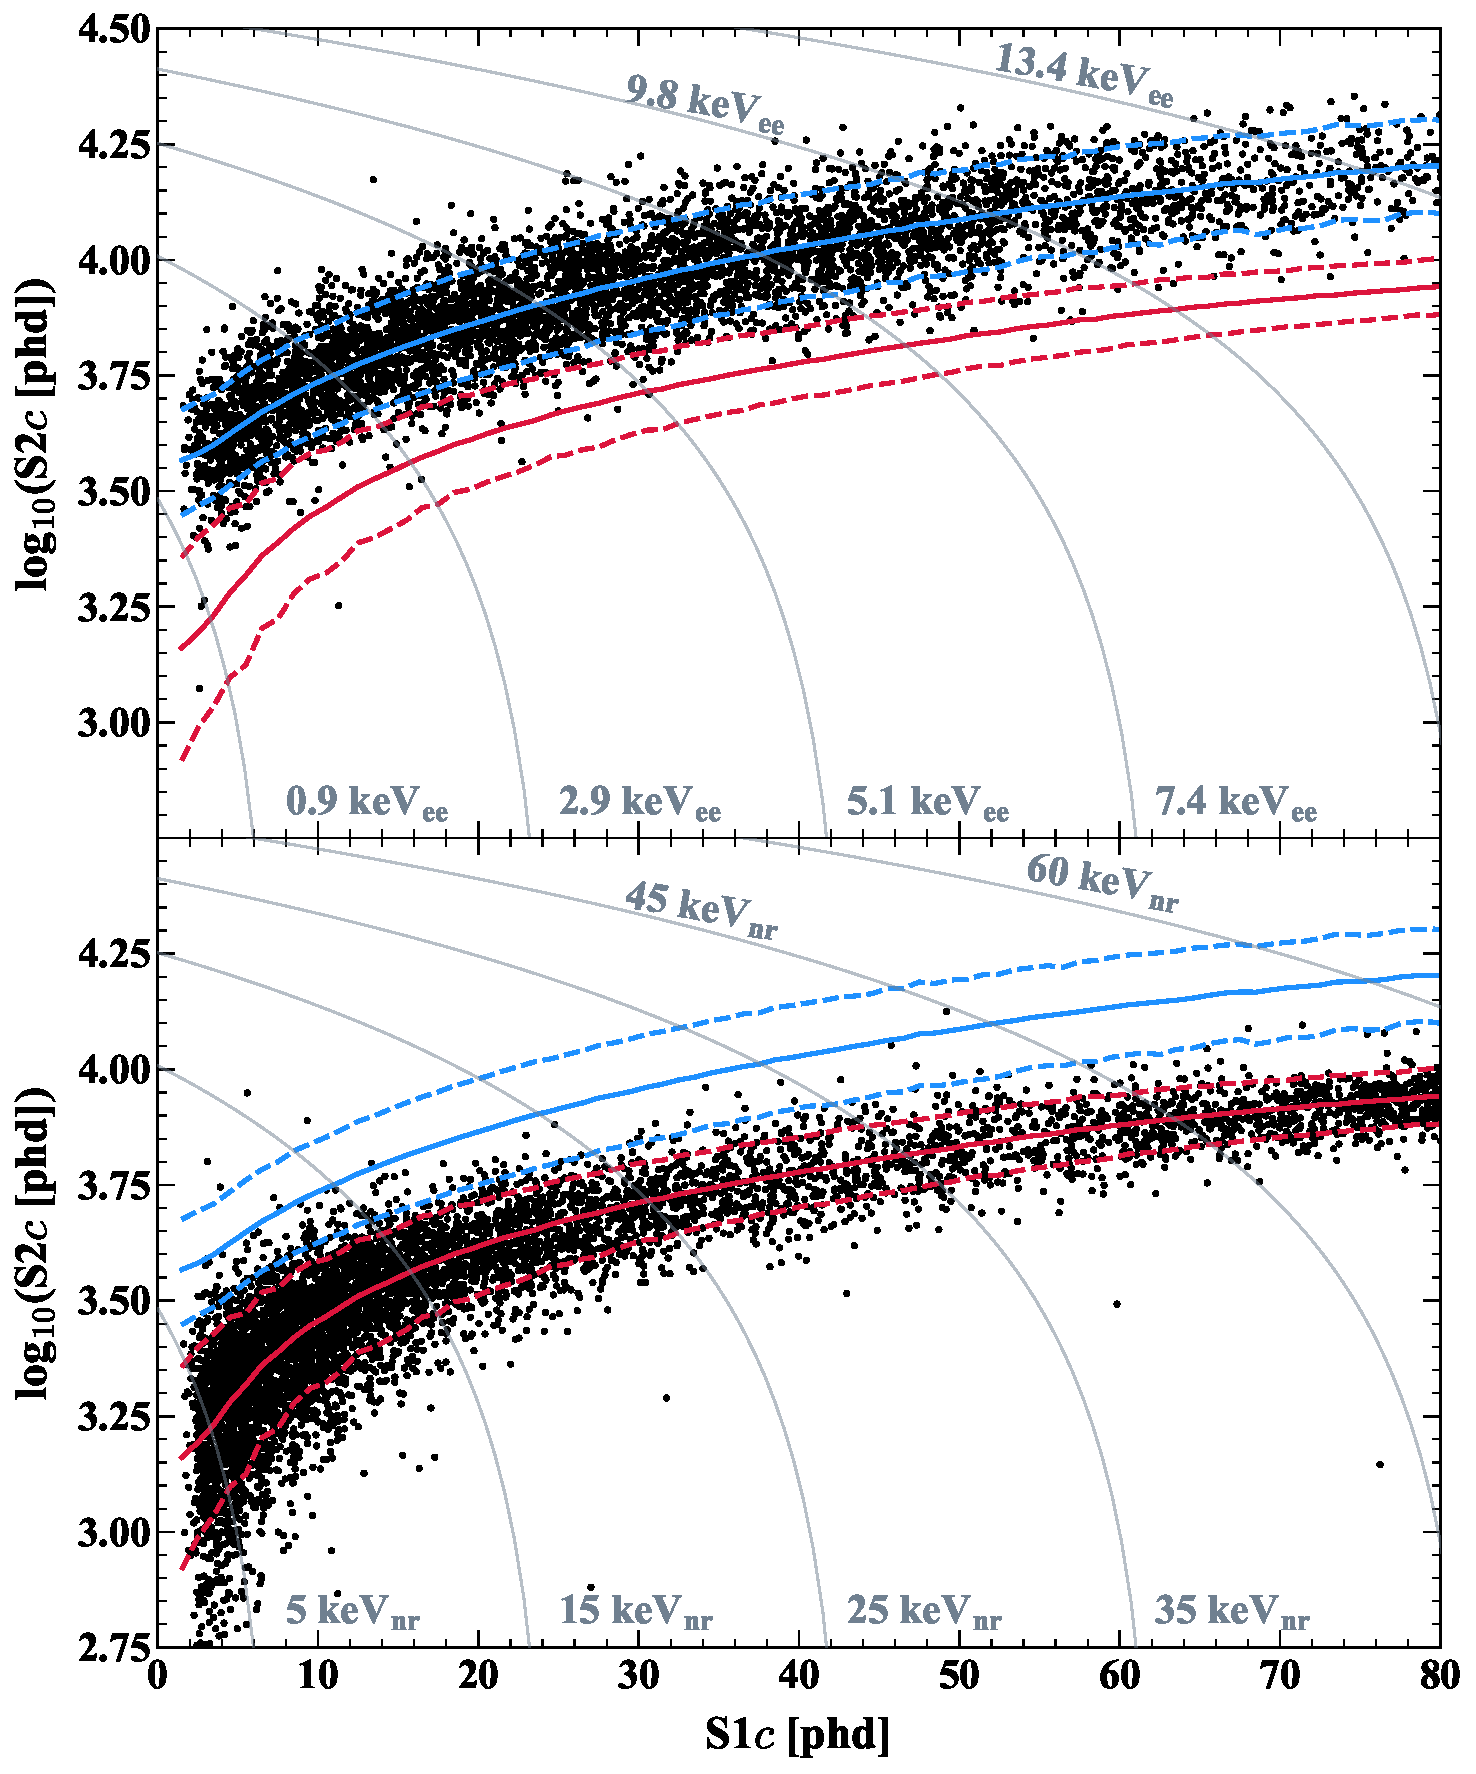
\includegraphics[width=10cm]{Figures/EFT/All_SR1_Plots/SR1WS_calOnly_0629_twoPanel.pdf}
    \caption{Calibration of ER and NR bands, shown in blue and red respectively.
             The solid line is the median and the dashed are the 10\% and 90\% quantiles.
             \textbf{Top:} ER events produced by $\beta$-decays from injected CH$_3$T.
             \textbf{Bottom:} NR events produced by DD neutrons.
             }
    \label{fig:sr1_tpc_calibration}
\end{figure}

\subsection{Analysis Cuts}
\par
In addition to the core-cuts that remove scatters that are inconsistent with dark matter that have been previously discussed, a multitude of other cuts were developed.
They fall broadly into three categories: live time, S2-based cuts and S1-based cuts.
These three, along with the core cuts are briefly discussed below.

\subsubsection{live time cuts}
The live time cuts are named as such as they have a large adverse affect on the amount of data that is uncharacteristic due to the high rate of pulses observed.
The two most significant cuts were an electron-train cut and a hot spot cut, together removing 35\% of the livetime.
After a large S2 event, a period of a sustained high rate is observed. 
This is due to electrons attaching to impurities and then being released at some later time, causing a delayed extraction and an elevated rate after the S2.
Single photons are also observed after the same event which is thought to be from delayed fluorescence.
The removal of time after an S2 until the detector rate settles corresponds to 29.8\% of live day loss.
Occasionally hot spots appeared in the TPC due to electron emission from the grids. 
These periods of time lasted approximately an hour at a time and reduced the live time by 6.6\%.
There were several other cuts in this category which combined livetime by a future 1\%.

\subsubsection{S2 cuts}
A suite of cuts were developed to remove S2s which did not look like an S2 should if it had originated from a LXe scatter.
These targeted accidental events.

\subsubsection{S1 cuts}


developed a hot spot where 

\subsubsection{Core cuts}
All of these core cuts focus on removing clean scatters in the TPC, but which do not match the properties of dark matter.
Only events with a single S1-S2 pulse pair are selected, multiple S1 or multiple S2 events are removed.
\par
The fiducial region was defined in $z$ by the drift time (time between the S1 and S2 pulses) of between [86,936.5] $\mu$s which corresponds to approximately 12.8 cm below the gate grid and 2.2 cm from the cathode grid.
$r$ was defined as either [4.0,5.0,5.2] cm from the TPC wall. The variation in the $r$ is to remove regions where the electric field is non-uniform, and effects from being close to the wall.
Within this region a the volume of xenon is 5.5$\pm$0.2 tonnes.
\autoref{fig:sr1_fiducial_cut} shows the fiducial volume definition.
\par
The region of interest was defined as 3 phd $<$ S1$_c <$ 80 phd, S2 $>$ 600 phd and S2$_c <$ 10$^5$ phd.
\par
The OD veto window was set to the value discussed in the previous chapter of 1200 $\mu$s, with an energy threshold of 200 keV.
The Skin veto window was set to 400 $\mu$s.
Additionally a prompt veto window was implemented to remove events where the S1 is within [-300,300] ns of a pulse in either the Skin or OD.

\par
The combined efficiency of all of these cuts is shown in \autoref{fig:sr1_nr_efficiency}.
The efficiency in the ROI was determined using AmLi and tritium data.
A total of 335 events remained after the application of all of these cuts.

\begin{figure}
    \centering
    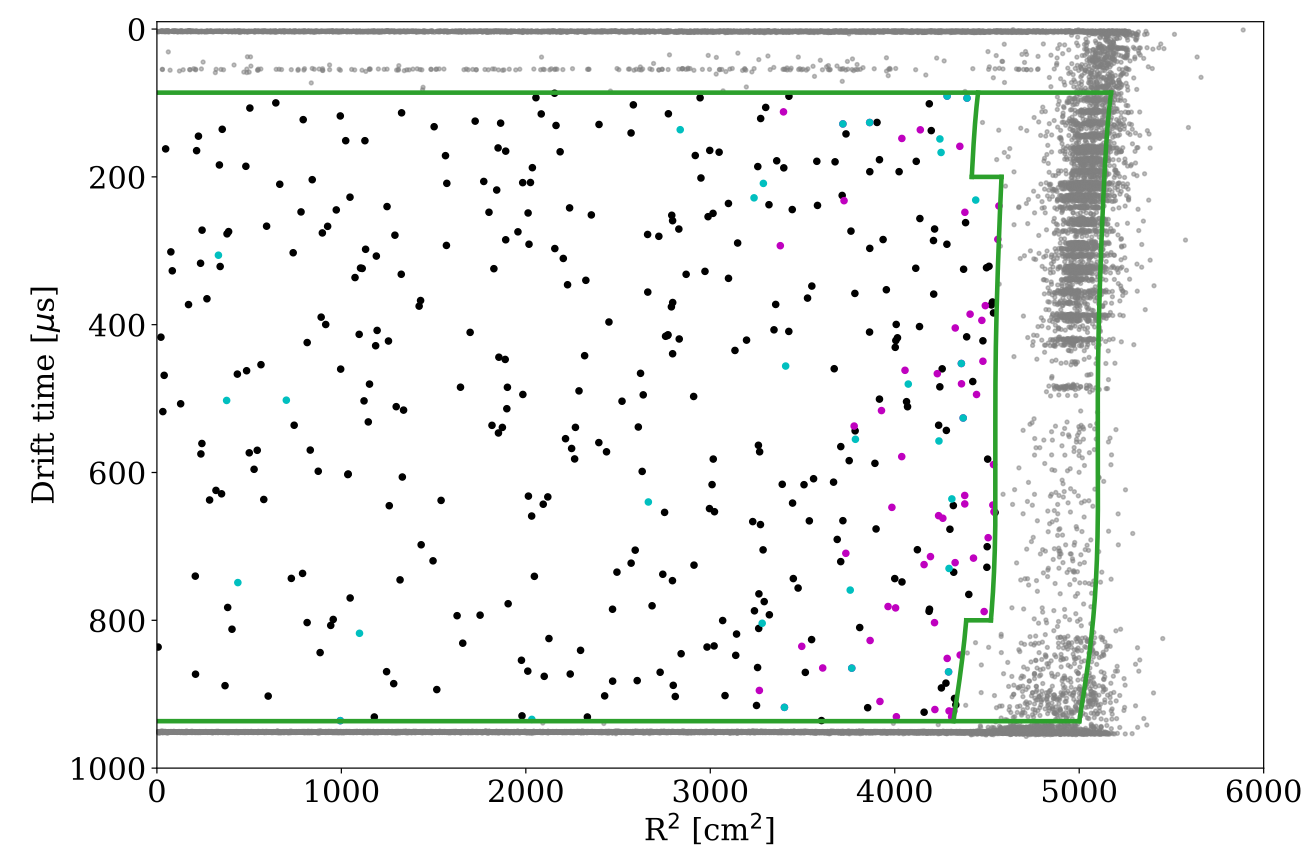
\includegraphics[width=15cm]{Figures/EFT/All_SR1_Plots/fid.png}
    \caption{Distribution of events in the SR1 dataset in the ROI.
    The vertical green line which two steps is the fiducial region.
    The other green line shown is the wall definition.
    The events in grey are outside of the fiducial volume and so vetoed. 
    The events marked in cyan were removed by the OD and the events marked in purple by the Skin.
    The remaining events in the WIMP dataset are shown in black.}
    \label{fig:sr1_fiducial_cut}
\end{figure}

\begin{figure}
    \centering
    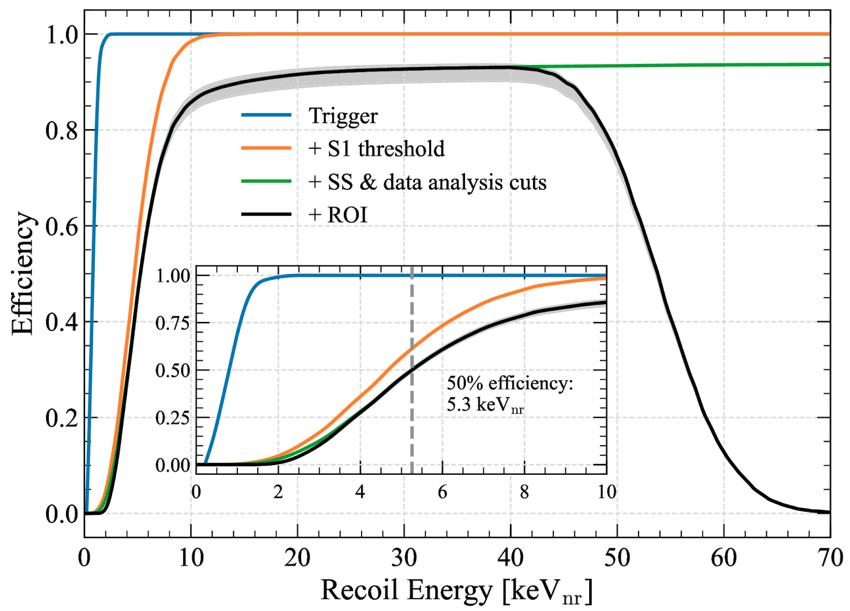
\includegraphics[width=10cm]{Figures/EFT/All_SR1_Plots/NR_efficiency.png}
    \caption{Signal efficiency as a function of NR energy for the trigger (blue), S1 threshold (orange), all analysis cuts expect ROI (green) and the ROI (black).
    The vertical dashed line is the the 50\% efficiency point.
    }
    \label{fig:sr1_nr_efficiency}
\end{figure}

\subsection{Background Model}
\par
In the background model, 9 components were included.
The grouping is based upon the distribution in the ROI and the level of uncertainty.

\par
The ${}^{222}$Rn chain and ${}^{220}$Rn chain both produce flat $\beta$ contribution.
The rate of these was determined via $\alpha$-peak fitting to the ER band outside of the ROI which can be seen in \autoref{fig:sr1_spectra}
The $\gamma$ spectrum from the detector contaminants is also flat in this region.
These contributions are treated as a single background labelled $\beta$ decays + Det. ER.
This is the largest contribution to the expected rate, with 218 $\pm$ 36 events.

The rate of detector 
\begin{figure}
    \centering
    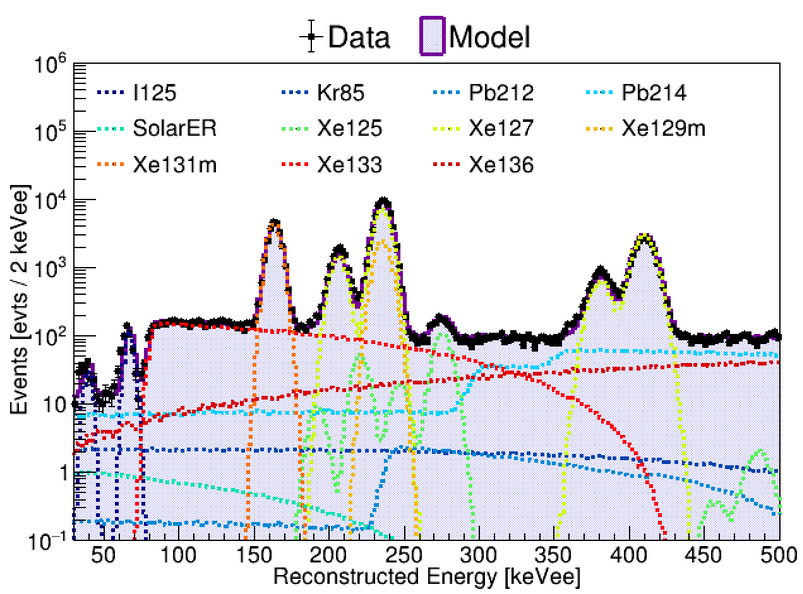
\includegraphics[width=10cm]{Figures/EFT/All_SR1_Plots/ER_band_fit.png}
    \caption{SR1 vanilla WIMP-search data (black points) overlaid on the background model.
    The contours shown for each distribution are 1 and 2 $\sigma$.
    ${}^{8}$B is shown in green, ${}^{37}$Ar is shown in orange, the combined ER spectrum in grey.
    The red lines are the NR band with the medium, 10\% and 90\% quantiles.
    The distribution from a 30 GeV WIMP is also shown in purple. 
    }
    \label{fig:sr1_spectra}
\end{figure}


\par
Solar neutrinos which also produce a flat contribution are not included as the rate is more finely constrained \cite{pp_solar_neutrinos_rate_ref}.
\par
Decays from three Xenon isotopes were included.
${}^{127}$Xe and ${}^{124}$Xe contribute to the ER spectrum by double electron capture and double $\beta$ decay respectively.
The rates of these are constrained by know abundances \cite{xenon_isotopes_ref}.
\par
Two interesting backgrounds considered here is weren't considered in the projected case are ${}^{37}$Ar and ${}^{127}$Xe.
These are both short-lived isotopes, with half-lives of 35 days and 36.3 days respectively.
They appear due to cosmogenic activation of the xenon when the xenon is at the surface level\footnote{of the mine. Not the surface of the LXe.}.
Once underground these components decay away and so are not of concern in future data runs.
The rates are therefore constrained by the delivery schedule of the xenon into the Davis cavern \cite{lz_argon37_ref}.
There are expected to be $\approx$100 ${}^{37}$Ar events in this data set but there a very large uncertainty meaning that it could be has high at 300.

\par
The two NR contributions considered are from ${}^{8}$B solar neutrinos and neutrons from the detector.
There are expected to be 0 detector neutrons in this dataset, a value constrained by the radioassay of the detector components prior to construction \cite{LZ_assay_ref}.

\par
The expected contribution from each component in the model is \autoref{tab:sr1_ws_lz_backgrounds}.
The uncertainties on the values shown indicate the constraints placed on each component during the PLR.

\begin{table}[]
    \centering
    \begin{tabular}{c|c}
        Background Component     & Expected Number of Events  \\ \hline
        $\beta$ decays + Det. ER & 218 $\pm$ 36 \\
        $\nu$ ER                 & 27.3 $\pm$ 1.6 \\
        ${}^{127}$Xe             & 9.3 $\pm$ 0.8 \\
        ${}^{124}$Xe             & 5.0 $\pm$ 1.4 \\
        ${}^{136}$Xe             & 15.2 $\pm$ 2.4 \\
        ${}^{8}$B CE$\nu$NS      & 0.15 $\pm$ 0.01 \\
        Accidentals              & 1.2 $\pm$ 0.3 \\
        ${}^{37}$Ar              & [0, 291]      \\
        neutrons                 & 0.0${}^{+0.2}$
    \end{tabular}
    \caption{Expected number of events from each component in the background model.}
    \label{tab:sr1_ws_lz_backgrounds}
\end{table}

\par
The best-fit background model is shown in \autoref{fig:final_data_points} with the the data set overlaid.
The best-fit values were identical to the SI result, as such the plot is shown from the SI result \cite{lz_ws_sr1_ref}.
The WIMP contours (shown in purple) are for a 30 GeV/c${^2}$ which is analogous to $\Operator$1 interactions of the same mass.

\begin{figure}
    \centering
    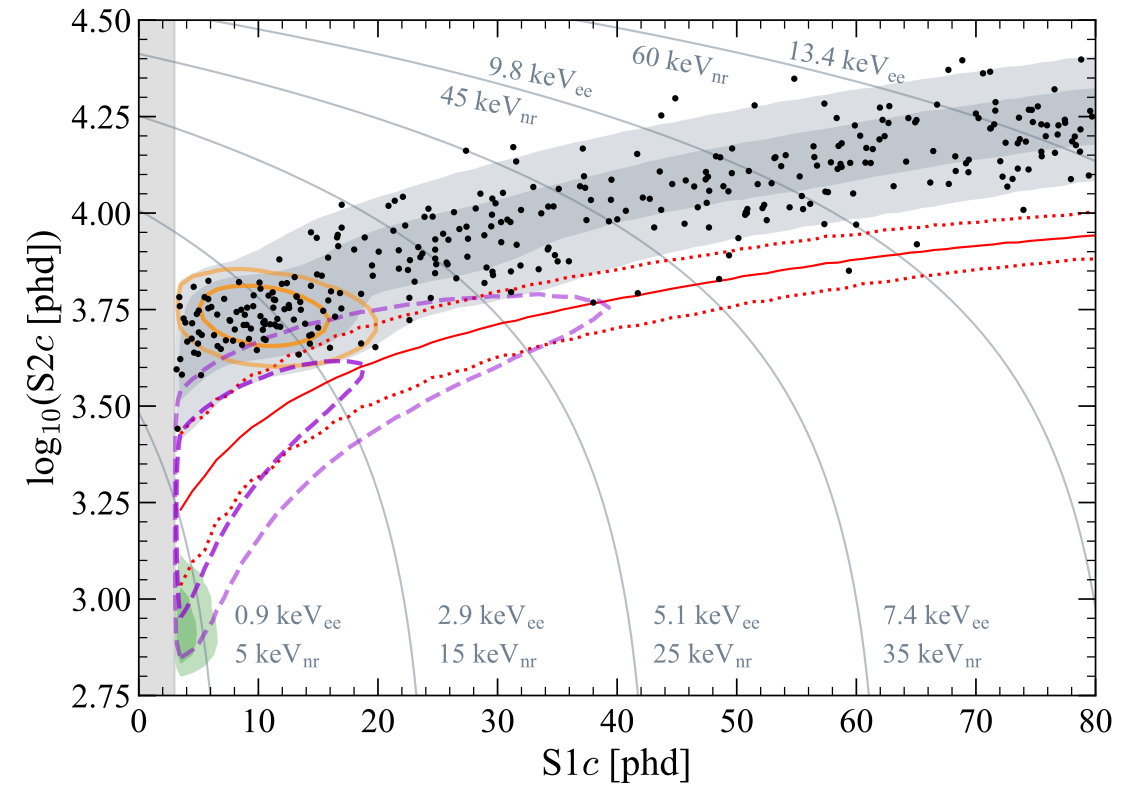
\includegraphics[width=10cm]{Figures/EFT/All_SR1_Plots/final_data_points.png}
    \caption{SR1 vanilla WIMP-search data (black points) overlaid on the background model.
    The contours shown for each distribution are 1 and 2 $\sigma$.
    ${}^{8}$B is shown in green, ${}^{37}$Ar is shown in orange, the combined ER spectrum in grey.
    The red lines are the NR band with the medium, 10\% and 90\% quantiles.
    The distribution from a 30 GeV WIMP is also shown in purple. 
    }
    \label{fig:final_data_points}
\end{figure}

\subsection{Signal Model}
\par
Unlike the projected sensitivity, this analysis used the recommended astronomic properties laid out in \cite{standard_halo_model_conventions_ref}.
These are summarised in \autoref{tab:sr1_DMFormFactor_parameters}.
Of particular note is the increased velocity of the WIMP velocity.
The impact of this on a selection of operator differential recoil rates is shown in FIGURE XXX.
\par
The increased velocity of the dark matter increased the flux, and therefore expected rate of recoils.
As the expected signal rate increases, the lack of seeing a signal then sets a tighter constraint on the WIMP-nucleon scattering.
A more complete comparison between how uncertainties in the standard model parameters affect sensitivity to dark matter searches can be found in \cite{LZ_Ibles_LZStats_Thesis_ref,billyboxer_thesis_ref}.

\begin{table}[]
    \centering
    \begin{tabular}{c|c}
        Parameter         & Value  \\ \hline
        $\nu_0$           & 238$km s^{-1}$ \\
        $\nu_{esc}$       & 544$km s^{-1}$ \\
        $\rho_{\chi}$     & 0.3 $GeV/cm^{3}$ \\
        $|\nu_E|$         & 245 $km s^{-1}$ 
    \end{tabular}
    \caption{Standard Halo Model parameters used for SR1 sensitivity study.}
    \label{tab:sr1_DMFormFactor_parameters}
\end{table}


\subsection{Limits}
\par
On each operator for WIMP masses of [5, 7, 10, 12, 14, 21, 33, 50, 100, 200, 400, 1000, 4000] GeV/c$^2$, a 2-sided frequentist confidence interval is determined above a 90\% confidence level.
Presented in \autoref{fig:EFT_Result_Projected_Sensitivity_1} and \autoref{fig:EFT_Result_Projected_Sensitivity_2} are the limits, presented in the same dimensionless form as the projected limits.
Shown as before are the previous limits from both Xenon100 \cite{xenon100_eft_ref} and LUX \cite{LUX_RUN4_EFT_2021}.

%Consistent with the SI and SD search, a null result was found, setting limits on the operator couplings.
%These are shown in \autoref{fig:EFT_Result_Projected_Sensitivity_1} and \autoref{fig:EFT_Result_Projected_Sensitivity_2} in the same dimensionless scale as the projected limits.

\par
World-leading sensitivity has been achieved for all operators at at least some masses.
In several cases, such as $\Operator$6 the sensitivity of LZ is less than that of both LUX and XENON100. 
This is due to the recoil distributions of these operators peaking outside of the ROI used here for high WIMP masses.
Despite this reduced parameter space, the huge increase in exposure has made LZ very competitive.

\begin{figure}[!htbp]%
\centering
\begin{tikzpicture}
\centering
    \begin{axis}[
            ylabel={log${}_{10}$(S2$_c$ [phd])},
            xlabel={S1 [phd]},
            width=15cm,
            height=8cm,
            ymin=2.75, ymax=4.5,
            xmin=0, xmax=80,
            ]
            
        \addplot[gray, opacity = 0.5, fill=gray]
            table [x=x, y=y]
            {Data/HENR/sr1_ws/sr1_data/beta_band_95.dat};
        \addplot[gray, fill=gray]
            table [x=x, y=y]
            {Data/HENR/sr1_ws/sr1_data/beta_band_68.dat};
    
        \addplot[green, opacity = 0.5, fill=green]
            table [x=x, y=y]
            {Data/HENR/sr1_ws/sr1_data/b8_band_95.dat};
        \addplot[green, fill=green]
            table [x=x, y=y]
            {Data/HENR/sr1_ws/sr1_data/b8_band_68.dat};
            
        \addplot[red, ]
            table [x=x, y=y]
            {Data/HENR/sr1_ws/nr_band.dat};    
        \addplot[red, dashed]
            table [x=x, y=high]
            {Data/HENR/sr1_ws/nr_band.dat};     
        \addplot[red, dashed]
            table [x=x, y=low]
            {Data/HENR/sr1_ws/nr_band.dat}; 
            
        \addplot[black, only marks,]
            table [x=S1c, y=log_10S2c]
            {Data/HENR/sr1_ws/ws_data.dat};
            
        \addplot[orange]
            table [x=x, y=y]
            {Data/HENR/sr1_ws/sr1_data/ar37_band_95.dat};
        \addplot[orange]
            table [x=x, y=y]
            {Data/HENR/sr1_ws/sr1_data/ar37_band_68.dat};
    \end{axis}
\end{tikzpicture}
    \caption{SR1 search data after all cuts.}
    \label{fig:henr_ws_sr1_events}
\end{figure}

For SR1 fewer parameters were taken into consideration with the PLR working in [S1,logS2] space.
Increasing the set of parameters will allow for improved discrimination and a potential discovery but runs into significant computational limitations as discovered in both \cite{nicolelarsen_thesis_ref, shaunalsum_thesis_ref, billyboxer_thesis_ref}, a different approach such as that described in \cite{flamenest_ref} and \cite{lux_ml_plr_ref} offer some hope for this.

\begin{figure}[!htbp]%
\centering
\begin{tikzpicture}
\centering
  \begin{groupplot}[view={0}{90},
    group style = {group size = 2 by 4,
                   vertical sep=1.5cm,
                   horizontal sep=2.0cm}]
    
    \pgfplotsforeachungrouped \x in {1,3,4,5,6,7,8,9}{
     \edef\tmp{
        \noexpand \nextgroupplot[
                                xlabel={Mass [GeV/c$^2$]},
                                ylabel=$({c}^{s}_{\x}\times{m}^{2}_{w})^{2}$,
                                mark size=0pt,
                                width=0.45\textwidth,
                                height=5.5cm,
                                xmode=log,
                                ymode=log,
                                yminorticks=true,
                                x label style={at={(axis description cs:0.75,-0.1)},anchor=near ticklabel},
                                y label style={at={(axis description cs:-0.13,.75)},anchor=near ticklabel},
                                ]
            
            
            
            \noexpand \addplot[green, name path = nsig1] table[x=mass, y=nsig1]
                      {Data/HENR/sr1_ws/Limits/O\x.dat};
                      
            \noexpand \addplot[green, name path = psig1] table[x=mass, y=psig1]
                      {Data/HENR/sr1_ws/Limits/O\x.dat};
                      
            \noexpand \addplot[yellow, name path = psig2] table[x=mass, y=psig2]
                      {Data/HENR/sr1_ws/Limits/O\x.dat};
            \noexpand \addplot[yellow, name path = nsig2] table[x=mass, y=nsig2]
                      {Data/HENR/sr1_ws/Limits/O\x.dat};
            
            \noexpand \addplot[yellow, forget plot] fill between[of=nsig2 and psig2];          
            \noexpand \addplot[green, forget plot] fill between[of=nsig1 and psig1];
            
            
            %\noexpand \addplot[black, name path = median] table[x=mass, y=median]
            %          {Data/HENR/Projected_Sensitivity/Results_method1/O\x.dat};
            
            \noexpand \addplot[black, dashed, name path = median] table[x=mass, y=median]
                      {Data/HENR/sr1_ws/Limits/O\x.dat};
            \noexpand \addplot[black, name path = median] table[x=mass, y=ucl]
                      {Data/HENR/sr1_ws/Limits/O\x.dat};     
                      
            \noexpand \addplot[blue, name path = xenon100] table[]
                      {Data/HENR/Xenon100/O\x.dat};
                        
            \noexpand \addplot[only marks, mark size=1, error bars/.cd,
                               y dir=both, y explicit, error bar style={color=black}]
                               table[x=mass,y=median, y error plus index=3, y error minus index=2] {Data/HENR/Projected_Sensitivity/LUX/O\x.dat};
        }
        \tmp 
        }
  \end{groupplot}
\end{tikzpicture}
\caption{}
\label{fig:EFT_Result_SR1_Sensitivity_1}
\end{figure}


\begin{figure}[!htbp]%
\centering
\begin{tikzpicture}
\centering
  \begin{groupplot}[view={0}{90},
    group style = {group size = 2 by 3,
                   vertical sep=1.5cm,
                   horizontal sep=2.0cm}]
    
    \pgfplotsforeachungrouped \x in {10,11,12,13,14,15}{
     \edef\tmp{
        \noexpand \nextgroupplot[
                                xlabel={Mass [GeV/c$^2$]},
                                ylabel=$({c}^{s}_{\x}\times{m}^{2}_{w})^{2}$,
                                mark size=0pt,
                                width=0.45\textwidth,
                                height=5.5cm,
                                xmode=log,
                                ymode=log,
                                x label style={at={(axis description cs:0.75,-0.1)},anchor=near ticklabel},
                                y label style={at={(axis description cs:-0.13,.75)},anchor=near ticklabel},
                                ]
            
                        
            \noexpand \addplot[green, name path = nsig1] table[x=mass, y=nsig1]
                      {Data/HENR/sr1_ws/Limits/O\x.dat};
                      
            \noexpand \addplot[green, name path = psig1] table[x=mass, y=psig1]
                      {Data/HENR/sr1_ws/Limits/O\x.dat};
                      
            \noexpand \addplot[yellow, name path = psig2] table[x=mass, y=psig2]
                      {Data/HENR/sr1_ws/Limits/O\x.dat};
            \noexpand \addplot[yellow, name path = nsig2] table[x=mass, y=nsig2]
                      {Data/HENR/sr1_ws/Limits/O\x.dat};
            
            \noexpand \addplot[yellow, forget plot] fill between[of=nsig2 and psig2];          
            \noexpand \addplot[green, forget plot] fill between[of=nsig1 and psig1];
            
            
            %\noexpand \addplot[black, name path = median] table[x=mass, y=median]
            %          {Data/HENR/Projected_Sensitivity/Results_method1/O\x.dat};
            
            \noexpand \addplot[black, dashed, name path = median] table[x=mass, y=median]
                      {Data/HENR/sr1_ws/Limits/O\x.dat};
            \noexpand \addplot[black, name path = median] table[x=mass, y=ucl]
                      {Data/HENR/sr1_ws/Limits/O\x.dat};     
                      
            \noexpand \addplot[blue, name path = xenon100] table[]
                      {Data/HENR/Xenon100/O\x.dat};
                        
            \noexpand \addplot[only marks, mark size=1, error bars/.cd,
                               y dir=both, y explicit, error bar style={color=black}]
                               table[x=mass,y=median, y error plus index=3, y error minus index=2] {Data/HENR/Projected_Sensitivity/LUX/O\x.dat}; 
                     
        }
        \tmp 
        }
  \end{groupplot}
\end{tikzpicture}
\caption{}
\label{fig:EFT_Result_SR1_Sensitivity_2}
\end{figure}

For SR1 fewer parameters were taken into consideration with the PLR working in [S1,logS2] space.
Increasing the set of parameters will allow for improved discrimination and a potential discovery but runs into significant computational limitations as discovered in both \cite{shaunalsum_thesis_ref, billyboxer_thesis_ref}, a different approach such as that described in \cite{flamenest_ref} and \cite{lux_ml_plr_ref} offer some hope for this.